% Extension 1: Cross-Dataset Robustness Slides

\begin{frame}{Extension 1: Cross-Dataset Robustness}
    \begin{columns}
        \column{0.5\textwidth}
        \textbf{Hypothesis:}
        \begin{itemize}
            \item Models learn \textbf{geometric circuits}
            \item Eigenvectors = ``Platonic forms'' (circularity)
        \end{itemize}
        
        \vspace{0.2cm}
        \textbf{Test Cases:}
        \begin{itemize}
            \item Writer Independence: MNIST $\leftrightarrow$ EMNIST-Digits
            \item Domain Transfer: MNIST $\rightarrow$ USPS
            \item Geometric Semantics: MNIST $\rightarrow$ EMNIST-Letters
        \end{itemize}
        
        \vspace{0.2cm}
        \textbf{Results:}
        \begin{itemize}
            \item MNIST $\to$ EMNIST: \textbf{97.7\%}
            \item MNIST $\to$ USPS: \textbf{72.3\%} (+19 pp)
            \item Letters: O$\to$0 (99.6\%), I$\to$1 (87.1\%), Z$\to$2 (88.8\%), S$\to$5 (87.4\%)
        \end{itemize}
        
        \footnotesize
        All models use CoM normalization
        
        \column{0.5\textwidth}
        \begin{figure}
            \centering
            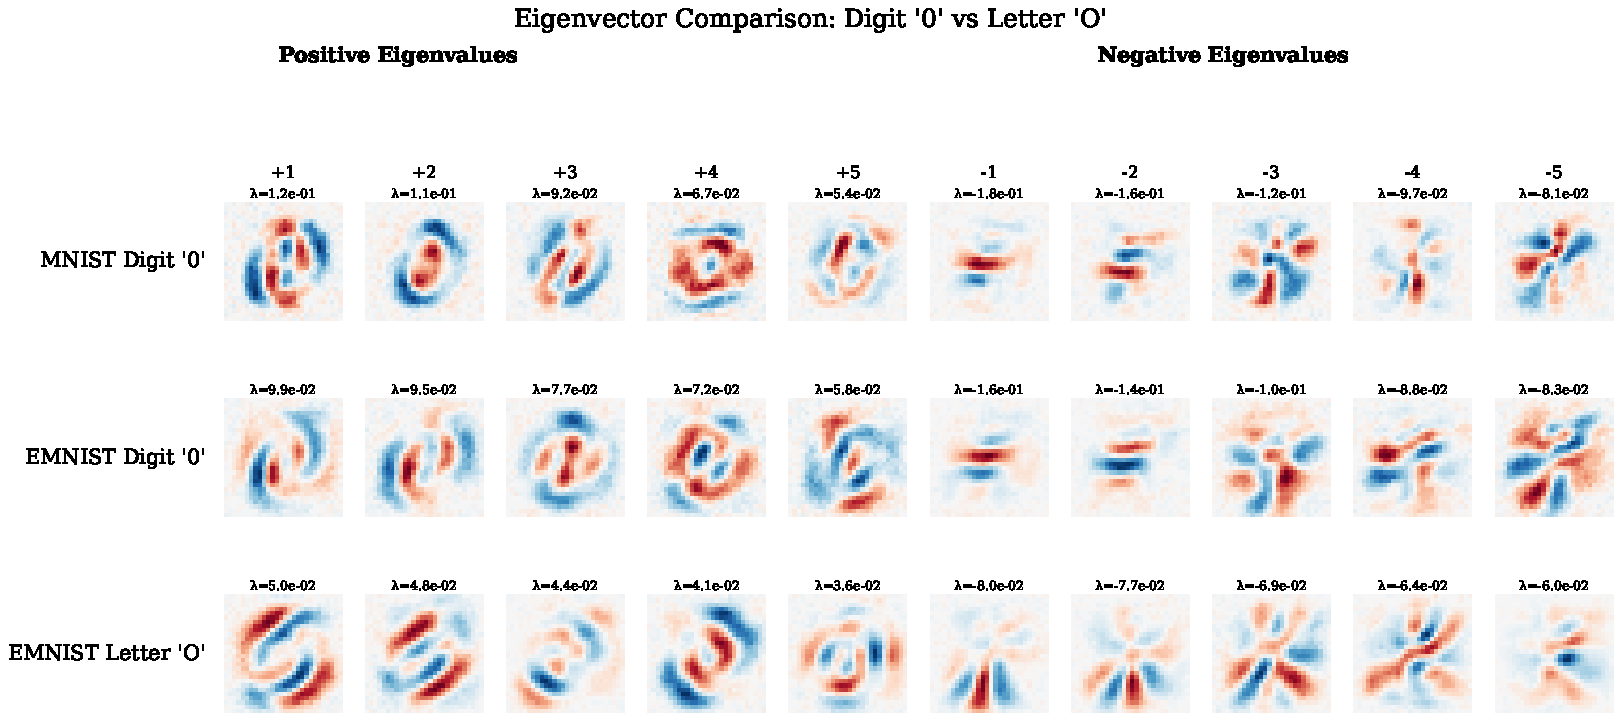
\includegraphics[width=0.95\textwidth]{../Report/figures/extension2/extension2_3way_comparison.pdf}
            \caption{Three-way eigenvector comparison}
        \end{figure}
    \end{columns}
\end{frame}

\begin{frame}{Quadratic Form Similarity}
    \begin{columns}
        \column{0.5\textwidth}
        \textbf{Problem: Cosine Similarity Fails}
        \begin{itemize}
            \item Similar (0--O): \textbf{0.358}
            \item Dissimilar (0--X): \textbf{0.339}
            \item Not discriminative!
        \end{itemize}
        
        \vspace{0.2cm}
        \textbf{Root Cause:}
        \begin{itemize}
            \item Shared eigenvector directions
            \item Class info in eigenvalue \emph{weights}
            \item Cosine ignores magnitudes
        \end{itemize}
        
        \vspace{0.2cm}
        \textbf{Solution:}
        \begin{equation*}
            \text{sim}(A, B) = \frac{\text{tr}(A \cdot B)}{\|A\|_F \|B\|_F}
        \end{equation*}
        
        \column{0.5\textwidth}
        \begin{figure}
            \centering
            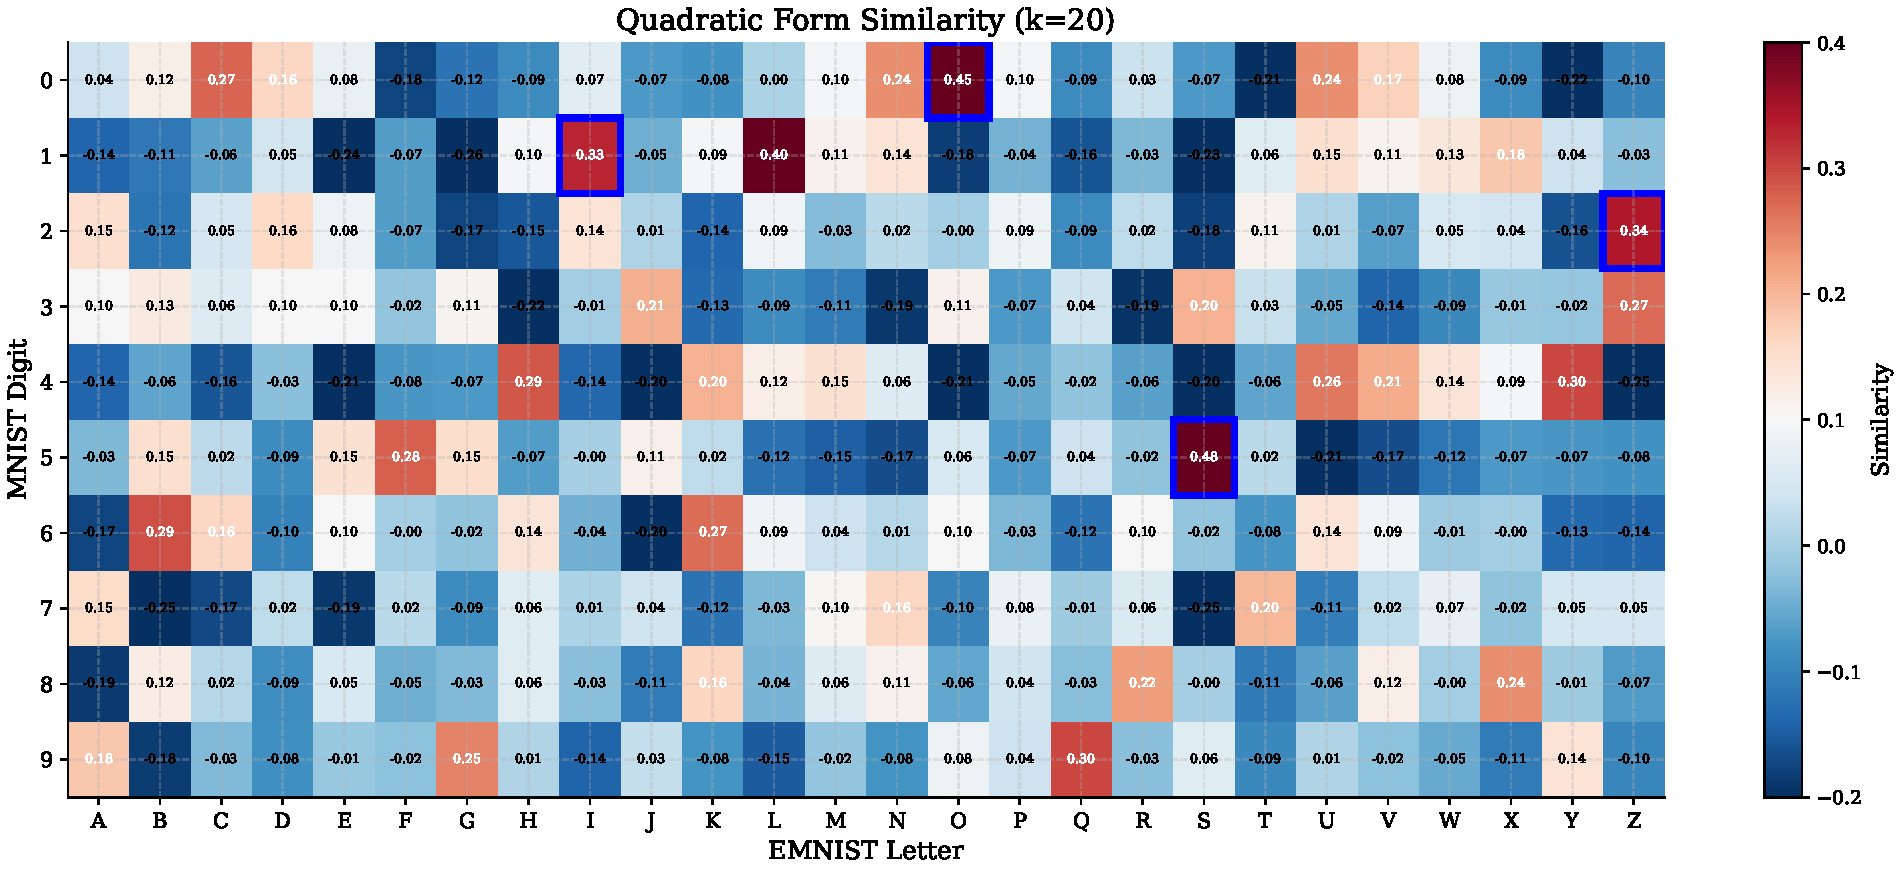
\includegraphics[width=0.95\textwidth]{../Report/figures/extension2/extension2_heatmap_quadratic_form.pdf}
            \caption{Quadratic Form Similarity heatmap}
        \end{figure}
        
        \vspace{0.2cm}
        \textbf{Results:}
        \begin{itemize}
            \item Similar: \textbf{0.400}
            \item Dissimilar: \textbf{-0.060}
            \item Gap: $p < 10^{-4}$
        \end{itemize}
        
        \footnotesize
        Incorporates eigenvalue signs and alignment
    \end{columns}
\end{frame}
